\section*{CHAPTER 2: BACKGROUND}
\addcontentsline{toc}{section}{\numberline{}CHAPTER 2: BACKGROUND}
\setcounter{section}{2}
\setcounter{subsection}{0}
\setcounter{figure}{0}
\setcounter{table}{0}

\subsection{OFDM Basics}

In digital communications, information is expressed in the form of bits. The term symbol refers to a collection, in various sizes, of bits. OFDM data are generated by taking symbols in the spectral space using M-PSK, QAM, etc, and convert the spectra to time domain by taking the Inverse Discrete Fourier Transform (IDFT). Since Inverse Fast Fourier Transform (IFFT) is more cost effective to implement, it is usually used instead \cite{b3}. Once the OFDM data are modulated to time signal, all carriers transmit in parallel to fully occupy the available frequency bandwidth. During modulation, OFDM symbols are typically divided into frames, so that the data will be modulated frame by frame in order for the received signal be in sync with the receiver. Long symbol periods diminish the probability of having inter-symbol interference, but could not eliminate it. To make ISI nearly eliminated, a cyclic extension (or cyclic prefix) is added to each symbol period. An exact copy of a fraction of the cycle, typically 25\% of the cycle, taken from the end is added to the front. This allows the demodulator to capture the symbol period with an uncertainty of up to the length of a cyclic extension and still obtain the correct information for the entire symbol period.

\begin{figure}[ht]
    \centering
    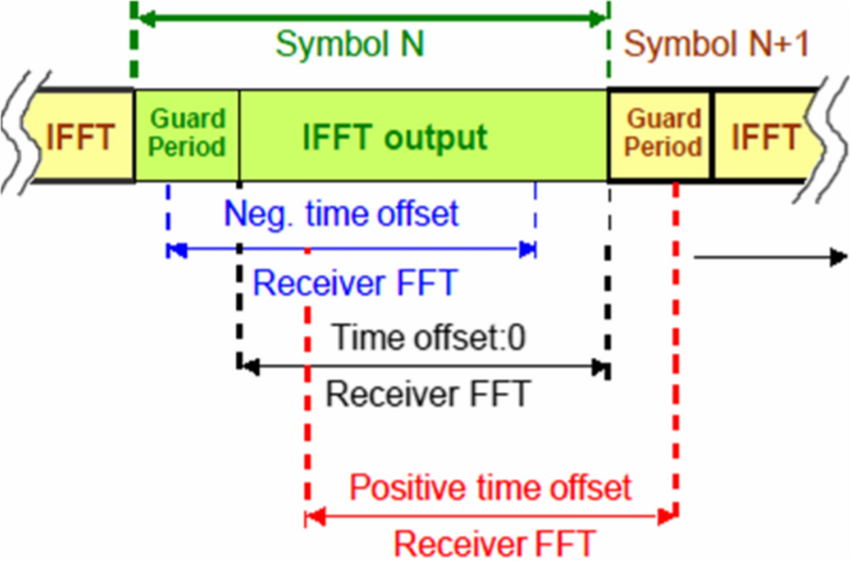
\includegraphics[width=0.5\textwidth]{Figures/Cyclic-extension-tolerance.png}
    \caption{\bfseries\centering\fontsize{13pt}{0pt}\selectfont Cyclic-extension-tolerance}
    \label{Cyclic-extension-tolerance}
\end{figure}

As shown in Figure \ref{Cyclic-extension-tolerance}, a guard period, another name for the cyclic extension, is the amount of uncertainty allowed for the receiver to capture the starting point of a symbol period, such that the result of FFT still has the correct information. In Figure 2, a comparison between a precisely detected symbol period and a delayed detection illustrates the effectiveness of the cyclic extension.

\begin{figure}[ht]
    \centering
    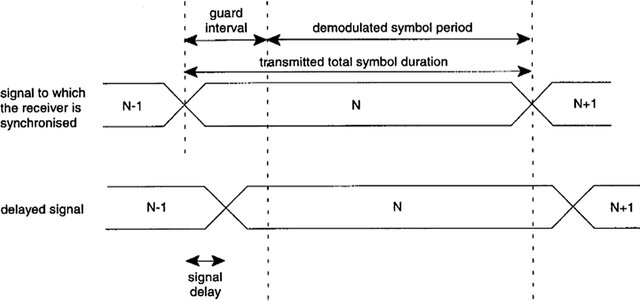
\includegraphics[width=\textwidth]{Figures/Effectiveness-of-cyclic-extension.jpg}
    \caption{\bfseries\centering\fontsize{13pt}{0pt}\selectfont Effectiveness-of-cyclic-extension}
    \label{Effectiveness-of-cyclic-extension}
\end{figure}

\subsection{OFDM Parameters and Characteristics}

\subsubsection{Complexity}

The number of carriers in an OFDM system is not only limited by the available spectral bandwidth, but also by the IFFT size, which is determined by the complexity of the system. The more complex (also more costly) the OFDM system is, the higher IFFT size it has; thus a higher number of carriers can be used, and higher data transmission rate achieved. The choice of M-PSK modulation varies the data rate and Bit Error Rate (BER). The higher order of PSK leads to larger symbol size, thus less number of symbols needed to be transmitted, and higher data rate is achieved. But this results in a higher BER since the range of 0-360 degrees of phases will be divided into more sub-regions, and the smaller size of sub-regions is required, thereby received phases have higher chances to be decoded incorrectly. OFDM signals have high peak-to-average ratio, therefore it has a relatively high tolerance of peak power clipping due to transmission limitations.

\subsubsection{Orthogonality}

The key to OFDM is maintaining orthogonality of the carriers. If the integral of the product of two signals is zero over a time period, then these two signals are said to be orthogonal to each other. Two sinusoids with frequencies that are integer multiples of a common frequency can satisfy this criterion. Therefore, orthogonality is defined by :

\begin{equation}\label{eq1}
    \int_{0}^{T} cos(2 \pi n f_o t) cos(2 \pi m f_o t) \,dt = 0 \quad (n \neq m) 
\end{equation}

Where $n$ and $m$ are two unequal integers; $f_o$ is the fundamental frequency; $T$ is the period over which the integration is taken. For OFDM, $T$ is one symbol period and $f_o$ set to to $\frac{1}{T}$ for optimal effectiveness.

\subsubsection{Advantages and Disadvantages}

Upgrading and optimizing algorithms, OFDM systems provide highly advantageous features for wireless transmission and transceiver system design:

\begin{itemize}
    \item  Complete Elimination of ISI (InterSymbol Interference): OFDM systems can entirely eliminate ISI by employing an appropriate Guard Interval, thus mitigating multipath distortion.
    \item Suitable for High-Speed Transmission Systems: OFDM is well-suited for high-speed transmission systems due to the significant reduction in Frequency Selectivity compared to single-carrier transmission. This reduction minimizes the impact of frequency-selective fading.
    \item Simple Receiver Structure: OFDM systems boast a simple receiver structure, contributing to ease of implementation.
\end{itemize}
However, OFDM technology also has its drawbacks that need careful consideration and practical research for designing a system suitable for specific purposes:
\begin{itemize}
    \item Uneven Amplitude Envelope: The amplitude envelope of the signal is uneven, causing nonlinear distortion in power amplifiers at the transmitter and receiver.
    \item Guard Interval Impact on Transmission Efficiency: While the guard interval is used to eliminate ISI, it also reduces transmission efficiency due to wasting power on transmitting useless signals.
    \item Orthogonality Conditions between Subcarriers: The requirement for orthogonality between subcarriers makes the system susceptible to the effects of Doppler, frequency offset, and time offset due to synchronization errors.
\end{itemize}
These challenges require careful consideration and research to optimize the performance of the OFDM system under real-world conditions and ensure that the drawbacks do not significantly affect transmission quality
